\documentclass[main.tex]{thesis.tex}
\begin{document}

\chapter{Apache Spark}

Apache Spark is an open source framework that combines an engine for distributing programs across clusters of machines with an elegant model for writing programs. \cite{ryza15}
Spark provides high-level APIs in Java, Scala, Python and R.

At a high level, every Spark application consists of a driver and one or more executors.
Driver is a program that runs the user's main function and executes various parallel operations on a cluster.
An executor is one machine in a cluster.

Spark can be introduced by describing its predecessor, MapReduce, and the advantages it offers.
MapReduce offered a simple model for writing programs that could execute in parallel across hundreds of machines.
MapReduce achieves nearly linear scalability as the data size increases.
The execution time is maintained by adding more computers to handle the task.

Spark preserves MapReduce's linear scalability and fault tolerance while extending it in three important ways.
First, in MapReduce the intermediate results between the map and reduce tasks must be written into memory where as Spark is able to pass the results directly to the next step in the pipeline.
Second, Spark treats the developers better by offering a rich set of transformations which enables users to represent complex pipelines in a few lines of code. (EXAMPLE?)
Third, Spark introduces in-memory processing by offering the Resilient Distributed Dataset (RDD) abstraction which offers a way for developers to materialize any step in a processing pipeline and store it into memory.
This means that future steps do not need to calculate the previous results again and they can continue a any intermediate step that the developer wants.
Previously this kind of feature has not been available within distributed processing engines. \cite{ryza15}

Spark programs can be written using Java, Scala, Python or R.
However, using Spark with Scala instead of Java, Python or R has a couple of advantages to it.
Performance overhead is reduced, since tasks such as transferring data across different layers or performing transformations for data may result in weaker performance.
Spark is written with Scala, which  has the implication that user has always access to latest and greatest features of the framework.
Spark philosophy becomes easier to understand when Spark is used with the language it was built with.
There is still one, maybe the biggest, benefit of using Scala with Spark, and it is the developer experience that comes with the fact that developer is using the same language for everything.
Importing data from database, data manipulation, shipping the code into clusters. \cite{ryza15}

Spark is shipped with a read eval print loop (REPL), which enables developers to test out things quickly in the console, without having to make the application self contained from the begin.
Usually when an application developed in REPL has matured enough, it is a good idea to move it into a compiled library (JAR).
This way it is possible to prevent code and results from disappearing.

\section{Resilient Distributed Dataset (RDD)}

A Resilient Distributed Dataset (RDD), is the main abstraction in Spark.
Essentially it is an immutable, partitioned collection of elements that can be distributed across multiple machines in a cluster. \cite{spark-rdd}

An important context to understand about RDDs is that they are lazy by nature.
When a new RDD is created, nothing is actually done, it means that spark knows where the data is when the time comes to do something with it.

RDD can be created in two ways: parallelizing an existing Scala collection in the driver program or referencing an external dataset in an external storage system, such as HDFS, HBase or any file system supported by Hadoop \cite{spark-programming-guide}.

RDDs can be persisted into memory, which allows programmer to reuse them efficiently across parallel operations.
RDDs are able to recover from node failures automatically, using Directed Acyclic Graph (DAG) engine.
DAG supports cyclic data flow.
Each Spark job creates a DAG of task stages to be performed on the cluster.
Compared to MapReduce, which creates a DAG with two predefined stages - Map and Reduce, DAGs created by Spark can contain any number of stages.
This allows some jobs to complete faster than they would in MapReduce, with simpler jobs completing after just one stage, and more complex tasks completing a single run of many stages, rather than having to be split into multiple jobs. \cite{mapRSpark}

\begin{figure}[h]
	\caption{Directed Acyclic Graph \cite{dag-image}}
	\centering
	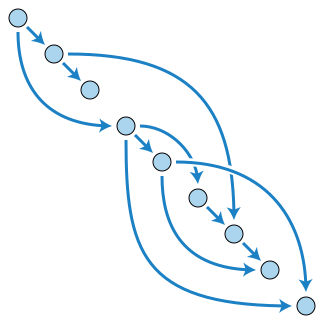
\includegraphics[scale=1.0]{directed_acyclic_graph}
\end{figure}

\section{Dataset API}
Dataset (DS) is the replacement for RDD in Spark.
It is a strongly typed collection of domain-specific objects that can be transformed in parallel using functional or relational operations.
Operations available on Datasets are divided into transformations and actions.
Transformations are operations such as map, filter, select and aggregate that produce new Datasets.
Actions are operations such as count, show, or writing data out to file systems that trigger computation and return results. \cite{spark-dataset}

Datasets are lazy by nature, which refers to that computations are only triggered when an action is invoked.
A Dataset essentially represents a logical plan that describes the computation required to produce the data.
Upon an action invocation, the query optimizer of Spark optimizes the logical plan and generates a physical plan for efficient execution in a parallel and distributed manner.
The logical plan as well as the optimized physical plan can be explored by using the $explain$ function. \cite{spark-dataset}

To efficiently support domain-specific objects, an Encoder is required.
The encoder maps the domain specific type T to Spark's internal type system.
For example, given a class Person with two fields, name (string) and age (int), an encoder is used to tell Spark to generate code at runtime to serialize the Person object into a binary structure.
This binary structure often has much lower memory footprint as well as is optimized for efficiency in data processing (e.g. in a columnar format).
To understand the internal binary representation for data, use the $schema$ function. \cite{spark-dataset}

Two ways typically exist to create a Dataset.
The most common way is to make use of the read function provided by SparkSession and point Spark to some files on the storage system:

\lstset{
	frame=0,
	language=Scala,
	breaklines=true,
}

\begin{lstlisting}[caption=Creating a new Dataset by using read function]

val people = spark.read.json("./people.json").as[Person]

\end{lstlisting}

where $Person$ would be a Scala case class, for example:

\begin{lstlisting}[caption=Definition of case class Person]

case class Person(id: BigInt, firstName: String, lastName: String)

\end{lstlisting}

Case classes are normal Scala classes that are:

\begin{itemize}
	\item Immutable by default
	\item Decomposable through pattern matching
	\item Compared by structural equality instead of by reference
	\item Succinct to instantiate and operate on
\end{itemize}

If we would omit the casting with keyword $as$ then we would end up creating a DataFrame and the schema of the created object would be guessed by Spark.

\begin{lstlisting}[caption=Creating a SparkSession]
val spark = SparkSession
  .builder
  .appName("MovieLensALS")
  .config("spark.executor.memory", "2g")
  .getOrCreate()
\end{lstlisting}

SparkSession is the entry point to programming Spark with the Dataset and DataFrame API. In the above snippet we create a $SparkSession$ by chaining calls to the builder method, which creates a SparkSession. Builder object for constructing a SparkSession. 
Datasets can also be created through transformations available on existing Datasets:

\begin{lstlisting}[caption=Creating a new Dataset through a transformation]

val names = people.map(_.name)

\end{lstlisting}

\cite{spark-dataset}

Datasets are similar to RDDs as they also provide strong typing and the ability to use powerful lambda functions \cite{spark-sql-programming-guide}. These are accompanied with the benefits of Spark SQL's optimized execution engine \cite{spark-sql-programming-guide}. However, instead of using standard serialization like Java serialization they use a specialized Encoder to serialize the objects.
Serialization denotes a task in which an object is turned into bytes thus reducing the memory footprint of the object.
In general, serialization is needed for processing or transmitting over the network.
While both encoders and standard serialization are responsible for turning an object into bytes, encoders are generated dynamically by code. They are using a format that allows Spark to perform many operations such as filtering, sorting and hashing without the need of deserializing the bytes back into an object. \cite{spark-programming-guide}

In the following listing, we create a new Dataset by reading a $json$ file from the file system. Next we create another Dataset through a transformation. We make use of the $copy$ method of Scala case class to clone an object, since we had declared the $people$ Dataset to be immutable. Finally, we display the physical plan by running the $explain$ function on the newly created Dataset.

\begin{lstlisting}[caption=Displaying the logical and physical plan of a Dataset]

val people = spark.read.json("./people.json").as[Person]
val peopleWithDoubleSalary = people.map { person => 
	person.copy(salary = person.salary * 2)
}
peopleWithDoubleSalary.explain

== Physical Plan ==
*SerializeFromObject [staticinvoke(class org.apache.spark.unsafe.types.UTF8String, StringType, fromString, assertnotnull(input[0, $line62.$read$$iw$$iw$Person, true], top level Product input object).name, true) AS name#212, staticinvoke(class org.apache.spark.sql.types.Decimal$, DecimalType(38,0), apply, assertnotnull(input[0, $line62.$read$$iw$$iw$Person, true], top level Product input object).salary, true) AS salary#213]
+- *MapElements <function1>, obj#211: $line62.$read$$iw$$iw$Person
+- *DeserializeToObject newInstance(class $line62.$read$$iw$$iw$Person), obj#210: $line62.$read$$iw$$iw$Person
+- *FileScan json [name#200,salary#201L] Batched: false, Format: JSON, Location: InMemoryFileIndex[file:/home/joonne/Documents/GitHub/thesis-code/people.json], PartitionFilters: [], PushedFilters: [], ReadSchema: struct<name:string,salary:bigint>

\end{lstlisting}

\section{DataFrame API}

Picture about rdd vs dataset vs dataframe ?

A DataFrame is essentially a Dataset that is organized into named columns.
In Scala, a DataFrame is represented by a Dataset of Rows.
It is conceptually equivalent to a table in a relational database or a data frame in R/Python, but it has richer optimizations under the hood.
DataFrames can be constructed from a range of sources such as structured data files, tables in Hive, external databases, or existing RDDs.
\cite{spark-sql-programming-guide}

\begin{figure}[h]
	\caption{DataFrame}
	\centering
	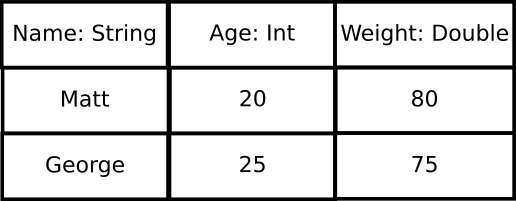
\includegraphics[scale=1.0]{dataframe}
\end{figure}

\section{Matrix Factorization}

Matrix factorization denotes a task in which a matrix is decomposed into a product of matrices.
There are many different matrix decompositions.
The following chapter will describe matrix factorization in general and the Alternating Least Squares algorithm which is the matrix factorization algorithm that is implemented in Spark.
It is based on same idea as Netflix prize winner, matrix factorization models.

Matrix factorization belongs to a vast class of algorithms called latent-factor models.
Latent-factor models try to explain observed interactions between a large number of users and products through a relatively small number of unobserved, underlying reasons.
For example, they can try to explain why people would buy a particular album out of endless possibilities by describing users and albums in terms of tastes which are not directly available as data. \cite{ryza15}
A latent factor is not available for direct observation. For example health of a human being is a latent factor.
Health can not be observed as a variable such as blood pressure.

\begin{figure}[h]
	\caption{Matrix factorization \cite{ryza15}}
	\centering
	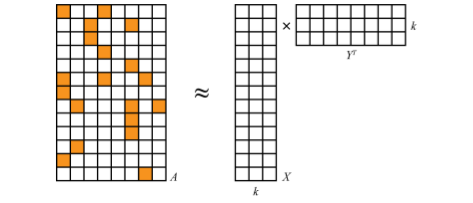
\includegraphics[scale=0.8]{matrix_factorization}
\end{figure}

Matrix factorization algorithms treat the user and product data as if it was a large matrix A.
Each entry in row $i$ and column $j$ represents a rating the user has given to a specific product. \cite{ryza15}

Usually $A$ is sparse, which denotes that most of the entries of $A$ are 0.
This is due to the fact that usually only a few of all the possible user-product combinations exist.

Matrix factorization models factor $A$ as the matrix product of two smaller matrices, $X$ and $Y$, which are quite tiny.
Since $A$ has many rows and columns, both of them have many rows, but both have just a few columns $(k)$. The $k$ columns match to the latent factors that are being used to explain the interactions of the data.
The factorization can only be approximate because $k$ is small. \cite{ryza15}

The standard approach to matrix factorization based collaborative filtering treats the entries in the user-product matrix as explicit preferences given by the user to the product, for example users giving ratings to movies.
Implicit data denotes for example page views or a value representing if a user has listened to a artist. Explicit data means actual ratings that a user has given to a product.
Spark ALS can handle both implicit and explicit data. \cite{spark14} \cite{ryza15}

Usually many real-world use cases have access only to implicit feedback data such as views, clicks, purchases, likes or shares.
However, instead of trying to model the matrix of ratings directly, the approach in Spark MLlib treats the data as numbers representing the strength of the observations such as the number of clicks, or the cumulative duration someone spent viewing a movie.
Instead of explicit ratings, these numbers are related to the level of confidence in observed user preferences.
Based on this data, the model tries to find latent factors that can be used to predict the expected preference of a user for an item. \cite{spark14}

Sometimes these algorithms are referred to as matrix completion algorithms.
This is because the original matrix $A$ may be sparse while the product $XY^T$ is dense.
Hence, the product is only an approximation of $A$. \cite{ryza15}

\subsection{Alternating Least Squares (ALS)}

Collaborative filtering is commonly used for recommender systems.
These techniques aim to fill in the missing entries of a user-item association matrix.
Spark MLlib currently supports model-based collaborative filtering, in which users and products are described by a small set of latent factors that can be used to predict missing entries.
Spark MLlib uses the Alternating Least Squares (ALS) algorithm to learn these latent factors. \cite{spark14}

Spark ALS attempts to estimate the ratings matrix A as the product of two lower-rank matrices, $X$ and $Y$. \cite{als14}

\begin{equation}
A = XY^T
\end{equation}

Typically these approximations are referred to as factor matrices.
The general approach is iterative.
During each iteration, one of the factor matrices is held constant, while the other is solved for using least squares. The newly-solved factor matrix is then held constant while solving for the other factor matrix. \cite{als14}
Spark ALS enables massive parallelization since it can be done separately, it can be done in parallel which is an excellent feature for a large-scale computation algorithm. \cite{ryza15}

Spark ALS is a blocked implementation of the ALS factorization algorithm.
Idea is to group the two sets of factors, referred to as $users$ and $products$, into blocks.
Grouping is followed by reducing communication by only sending one copy of each user vector to each product block on each iteration.
Only those user feature vectors are sent that are needed by the the product blocks.
Reduced communication is achieved by precomputing some information about the ratings matrix to determine the out-links of each user and in-links of each product.
Out-link denotes those blocks of products that the user will contribute to.
In-link refers to the feature vectors that each product receives from each user block they depend on.
This allows to send only an array of feature vectors between each user block and product block.
Consequently the product block will find the users' ratings and update the products based on these messages. \cite{als14}

Essentially, instead of finding the low-rank approximations to the rating matrix $A$, it finds the approximations for a preference matrix $P$ where the elements of $P$ are $1$ when $r > 0$ and $0$ when $r <= 0$.
The ratings then act as confidence values related to strength of indicated user preferences rather than explicit ratings given to items. \cite{als14}

\begin{equation}
A_iY(Y^T Y)^{-1} = X_i
\end{equation}

Alternating Least Squares operates by rotating between fixing one of the unknowns $u_i$ or $v_j$.
While the other is fixed the other can be computed by solving the least-squares problem.
This approach is useful because it turns the previous non-convex problem into a quadratic that can be solved optimally \cite{aberger14}.
A general description of the algorithm for ALS for collaborative filtering taken from \cite{aberger14} is as follows:

\begin{lstlisting}[caption=Alternating Least Squares algorithm \cite{aberger14}]

1. Initialize matrix V by assigning the average rating for that movie as the first row, and small random numbers for the remaining entries.

2. Fix V, solve U by minimizing the RMSE function.

3. Fix U, solve V by minimizing the RMSE function.

4. Repeat Steps 2 and 3 until convergence.

\end{lstlisting}

Minimizing the Root Mean Square Error RMSE function denotes a task in which line is plotted. EXPLAIN RMSE.

\end{document}